
%\chapter{chapter}
%\section{section}
%\subsection{subsection}
%\subsubsection{subsubsection}
%\paragraph{paragraph}
%\subparagraph{subparagraph}

\begin{quote}
    \textit{In the boundless universe of literature there are always new avenues to be explored, both very recent and very ancient, styles and forms that can change our image of the world … But if literature is not enough to assure me that I am not just chasing dreams, I look to science to nourish my visions in which all heaviness disappears.}\\
    -Italo Calvino, \textit{Six Memos for the Next Millennium}
\end{quote}

\begin{quote}
    \textit{I am the angel who dwells in the point where the lines fork. Whoever retraces the way of divided things encounters me, whoever descends to the bottom of contradictions runs into me, whoever mingles again what was separated feels my membraned wing brush his cheek!}\\
    -Italo Calvino, \textit{The Castle of Crossed Destinies}
\end{quote}

Narrative games are a rich subset of interactive media, concerned with and focused around communicating a story, to which other aspects and systems of the game are in service. As forms have matured through the years, so has the complexity and dynamism of these systems. In both commercial and independent games, creators have turned to dynamic narrative systems to offer experiences that are more reactive to player actions, more responsive and reactive to game state, and thus more compelling. Players have also come to expect more from the stories told in games, and so there's a push to create more dynamic and reactive narratives, requiring more sophisticated systems needed to tell them.

Game designers turn to dynamic narrative systems for specific reasons. Perhaps they want players to experience a sense of agency and control through making choices at key narrative points, as in Telltale \cite{telltale} and Quantic Dream games \cite{quantic}. Perhaps they want players to experience a feeling of agency, but through affecting the gameplay system (which in turn affects the narrative) such as in simulationist works like \textit{King of Dragon Pass} and its sequel, \textit{Six Ages} \cite{dunham}.

Or they may be in a position where the dynamism of the narrative system isn't necessarily the focus, but is an emergent requirement from the narrative needing to support reactive and dynamic gameplay, such as in a game with dynamic quests like \textit{Skyrim}'s ``Radiant Story" system \cite{bertz_2011}. And a focus on games (and other interactive forms) should not cause us to lose sight of other related areas, such as work in which the story is predicated on dynamic narrative systems, even though they are not interactive or directly player-facing, such as \textit{The Annals of the Parrigues} \cite{short_2015} and other works within the NaNoGenMo community \cite{kazemi}, or locative literature works such as Hight et al's \textit{34 North 118 West} \cite{hight_knowlton_spellman}.

\section*{The Problem}

These approaches are not without their attendant problems. The main issue, as one might expect, stems from the demands of the systems providing the interactivity. Simply put, writing content for these systems is labor-intensive. The more dynamic, the more expansive the interactivity, the more content required to surface that. And if not properly accounted for in the design of these systems, creating and designing that content can easily become a task that dwarfs by far the content challenges from concomitant non-dynamic forms.

Furthermore, even if dynamic content is designed to broadly cover more interactions, and is reusable in different situations, it incurs another problem: authoring complexity. Simply put, authoring said dynamic content can be so complex it slows production until the game's total content could have been authored faster using simpler, static methods, even though the volume of content needed would be much higher.

Systems in this situation, where static content authoring is still more efficacious than dynamic, are being blocked by the ``authoring wall," and will be fighting an uphill battle until they overcome it.

\section*{The Authoring Wall}
\label{authoring-wall}

The authoring wall is a term used to describe the barrier for static systems (narrative or otherwise) to achieve some measure of systemic dynamism. Mateas et al. \cite{mateas2012artificial} used it to describe how traditional game development practices could not support authoring to the level required for experiences with high levels of dynamism. In contrast, AI development practices, while requiring more authoring effort up front, over time ``top out" with a still-bearable authorial burden, which allows them to push past the authorial wall into more dynamic territory (Figure \ref{fig:authoringWall1}A).

The authoring wall in this case is the point where--for static authoring systems, despite huge amounts of expended effort--only a moderate amount of dynamism is added. Concomitantly, there is a second line of demarcation in this graph, which could be called the ``complexity ceiling." This is the line of highest authorial effort the dynamic system requires, while continuing to provide added dynamism as authoring continues. A modified version of Figure \ref{fig:authoringWall1}A with these two demarcating lines can be seen in Figure \ref{fig:authoringWall1}B.

%%%%%%%%%%%%%%%%%%%% Figure/Image starts here %%%%%%%%%%%%%%%%%%%%
\begin{figure}
    \centering
    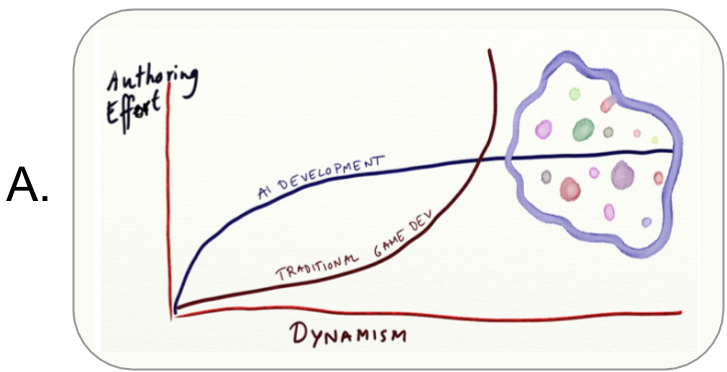
\includegraphics[width=\textwidth]{figures/1A.png}
    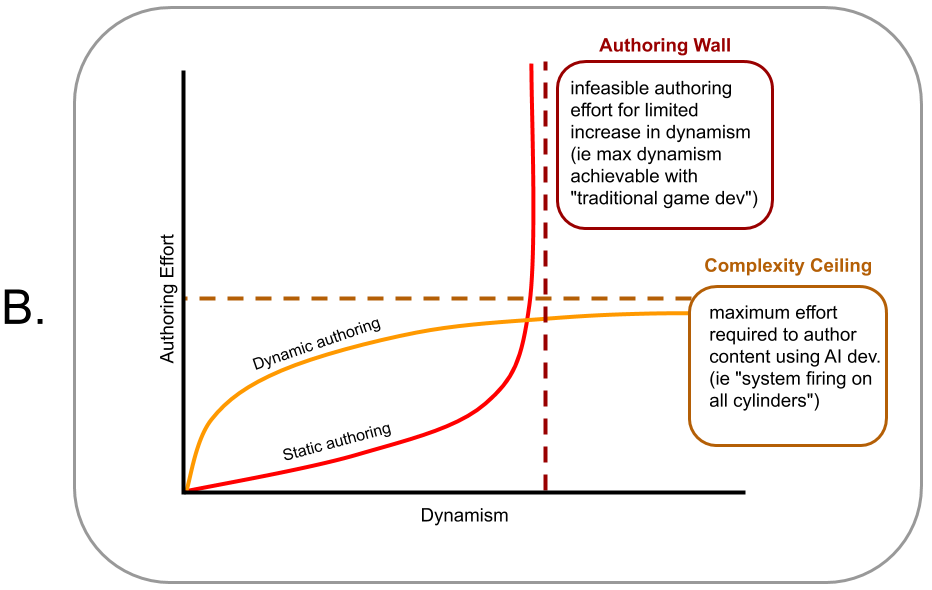
\includegraphics[width=\textwidth]{figures/1B.png}
    \caption{A: Original graph from \cite{mateas2012artificial} As ``traditional game dev approaches" increase dynamism, the authoring effort increases asymptotically. \newline B: Modified graph. The line of dynamism these static systems struggle to pass is the ``authoring wall", which ``AI development" can pass. The level of authoring effort AI dev asymptotically approaches is what could be called the ``complexity ceiling." Systems should seek to lower the ``complexity ceiling" through the use of authoring tools, and pass the authoring wall for a concomitant static system quickly by leaning into the unique affordances of their dynamic system.}
    \label{fig:authoringWall1}
\end{figure}
%%%%%%%%%%%%%%%%%%%% Figure/Image 1 Ends here %%%%%%%%%%%%%%%%%%%%



%%%%%%%%%%%%%%%%%%%% Figure/Image starts here %%%%%%%%%%%%%%%%%%%%
\begin{figure}
    \centering
    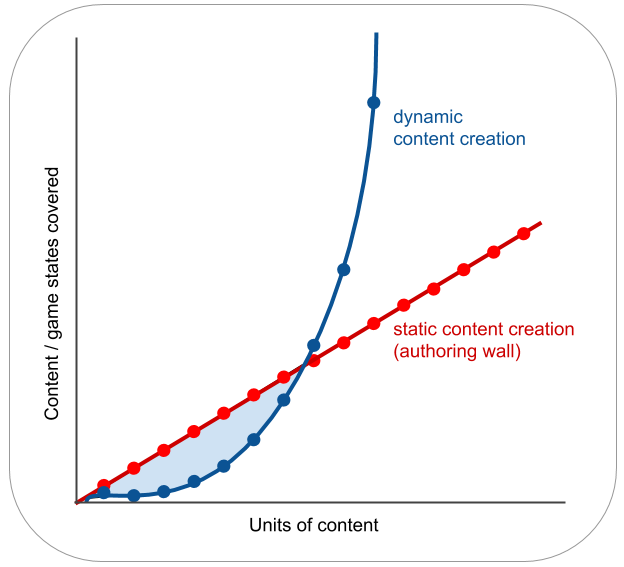
\includegraphics[width=8.5cm]{figures/2.png}
    \caption{Desired performance of dynamic systems when compared to static. While they may underperform initially, their dynamism allows them to cover more states eventually, and the performance gains (hopefully) far outstrip the initial underperformance, enabling new media experiences.}
    \label{fig:authoringWall2}
\end{figure}
%%%%%%%%%%%%%%%%%%%% Figure/Image 1 Ends here %%%%%%%%%%%%%%%%%%%%

These graphs are good at illustrating the interplay between ``effort" and ``dynamism." Another way to look at it is through the lens of content unit production (Figure 2). The authoring wall in this case is the static content creation strategy, which is specific to the system and experience being considered. The static authoring approach always makes incremental progress for each piece of content added, but never sees any increase in game state coverage due to system dynamics. The key interplay here is that, while dynamic systems may require more units of content to initially cover game states (and thus require more effort than static methods) over time that authoring compounds, which allows dynamic systems to exploit those gains to cover more game states than the more ``manual approach" required by static content creation. Ideally, in time the gains made from this ``compounded coverage" outstrip static approaches by so much that they functionally enable new types of media experiences that otherwise wouldn't be possible.

Alternatively, the area below the static version of the authoring wall can also be where the authoring time for a dynamic piece of content fulfilling some number of cases is greater than the time it would take to author enough static content to fulfill the same number of cases. For example, a dynamic unit of content that covers 10 games states but takes an hour to write is ``slower" than 10 units of static content that cover one state per piece and can all be written in half an hour.

Conversely, to be considered past the wall, authoring one piece of dynamic content needs to be either faster, or cover more cases than the time it would take to statically author for the same number of cases.

Regardless which of these two lens is used to view it, overcoming the authoring wall requires careful planning and design. This isn't meant as proscriptive for all dynamic narrative works: too much structure early on may stifle creativity for some practitioners, and the benefits of content planning may not outweigh the loss in creative output in some cases. Similarly, dynamic narrative content may seem like a natural fit for some projects, or a potentially exciting bell-and-whistle, when the reality of the design is one which can be satisfied with static content more reliably. 

However, for some types of dynamisms, systems are necessary to provide the project's required breadth and depth of content reactivity. By extension, leaning into the strengths of said systems when creating dynamic content yields more useful content than what could be obtained through static authoring alone. Furthermore, surfacing the system's capabilities to the player through the content provides a unique affect that can both help guide the player's interactions by signposting the types of interactions it excels at, and better communicate the story it's trying to tell. And for projects looking to keep to a deadline or guard against scope creep, understanding the project's authoring wall is a critical part of the design process.

Critically, where the authoring wall exists is not simply a function of the technical system, but hinges heavily on the narrative design of the experience authored with the system. Generally speaking, if the narrative design of the experience is leaning into the strengths of the system, the authoring wall is passed quicker. And the more dynamic the system and design, in general the further out the wall will be (requiring more authoring up front), but the greater the leverage once you're past the wall. 

Similarly, good design for these dynamic systems should be one where a static version of the same content very quickly becomes infeasible, because that demonstrates that the dynamisms enabled by the system are being exploited successfully to create a unique experience. If far into a project the static authoring method is still providing a competitive solution to that of the system, re-evaluation of the content design should be considered.

And while there is a rich seam of academic research in the creation of dynamic narrative systems and their attendant challenges, too often the concomitant \textit{design} challenges are not addressed or developed with equal footing. These systems may enable amazing interactive experiences, but creating a first-class game or media experience with them is often untenable. Some require incredibly technical skills to create one piece of content, which makes the per-unit time discouragingly high. Some allow fast authoring, but need such a large amount of content that authoring it in necessary volume requires a time commitment that is discouragingly high.

\section*{The Value of Content Creation For Research}

Critically, in these comparisons we are assuming ``surface text quality parity" between static hand-authored content and dynamic content, and that the quality level is that of a fully realized narrative experience. While an argument could be made for sacrificing the quality of content for an exchange in dynamism, in general any provisional authoring not meeting the quality standards for a fully-realized experience is setting itself up for more of a theoretical, research-focused experience creation. Because we are concerned with new forms of interactive narrative that can be experienced as fully realized experiences in their own right, in this dissertation we will be focused on authorial issues as they apply to this goal of polished output, as opposed to more provisional content used in research focused more primarily on system dynamics, with less a mind for what experiences using it might entail.

This focus was chosen because, in our experience, these dynamisms (and their attendant problems) only emerge during authoring of fully realized content, exposing weaknesses or blind spots rooted in assumptions of the underlying system. Because of this, development of dynamic narrative systems can't be considered pragmatically complete until exemplary content is authored with them. Therefore, the development of even theoretical interactive narrative systems can still introduce new concomitant procedural design and content authoring strategies. These strategies, even if unique to their corresponding system, represent paired first-class research contributions.

This stance is one that has been shared by other researchers in the field for quite some time, spurred by calls to make ``this powerful new medium for multiform narrative as expressive of the writer’s voice as is the printed page" \cite[250]{hamlet_holodeck}, concern over the resultant combinatorial explosion such experiences entail \cite{combo_stern}, the need for humanities-style analysis of the media artifacts resulting from such systems \cite{koenitz_five_theses}, and calls for new methods of research evaluation that can take into account the contributions from not just ``demonstrations", but also ``projects" and fully-fledged ``products" \cite[63-64]{wardrip2014envisioning}.

Thus we have narrative systems, which provide grounded solutions to technical problems, paired with content authoring strategies, which provide solutions to the authoring space problem each system poses. Unifying both, and treating the authoring insights as first-class research results alongside the system, allows us to increase the utility of the developed systems, by providing guides for playing to their strengths, and avoiding their particular pitfalls. Furthermore, these authoring insights may be generalizable to other systems, and used to overcome recurring problems when authoring dynamic content.

This position is one which was adopted over the course of six years of research into dynamic narrative systems, paired with media experiences that helped ground them in the pragmatics of content creation. Doing so has brought us up sharply against the Authoring Wall in different contexts, and from the different strategies used to engage and overcome it, the Authorial Leverage framework was abstracted.

\section*{Authorial Leverage}

Broadly speaking, these system-specific design insights have a common goal: maximization of authorial leverage. Thus, having a framework to characterize content creation with high authorial leverage is useful to drive development of the systems, and evolve them further as content is created with them.

Authorial leverage was first formally defined by Chen et al as ``the power a tool gives an author to define a quality interactive experience in line with their goals, relative to the tool’s authorial complexity" \cite{chen2009evaluating}, although previously used by Strong \cite{strong2008talking} to talk about combinatoric authoring, and simply as ``leverage" by Mateas when discussing semiotic systems that facilitate authoring for complex systems \cite{mateas2003expressive}.

For our purposes, it's useful to break down authorial leverage further, and center it on the pragmatics of dynamic narrative production. For ambitious systems with lots of state space and dynamism, greater authorial leverage means both being able to surface that state space to the player, and cover the necessary dynamic points, all without breaking the back of the writers or the project's budget (which effectively translates into labor as well). Knowing what factors play into authorial leverage can help us profile and evaluate system designs, in order to avoid situations where the amount of authoring is infeasible to accomplish the experience's goals.

To this end, we're concerned with two main components of authorial leverage: traversability (which is the scope of the dynamism presented to the player, and how content is deployed to accomplish that) and authorability (the system's requirements for content creation). Each has their own breakdown of important questions necessary to keep in mind when designing dynamic narrative systems.

\subsection{Traversability}

Before we can talk about creating content for an experience, we need to first understand the breadth and depth of what we're trying to achieve. Because this is a pragmatic framework, centered on the experience as the end-goal, our overarching question is: how much of the authored content is seen by the player by the time they have finished playing the game? 

This breaks down into the following four categories of questions:

\begin{itemize}
	\item \textbf{Explorability}: how many content pieces does the player see in one complete playthrough? 
	\item \textbf{Replayability}: how many playthroughs is the player expected to undertake?
	\item \textbf{Reusability}: how many situations could an authored piece of content be reused in different contexts in a playthrough? How many different prospective playthroughs could content reappear in?
	\item \textbf{Contextuality}: how reactive/dependent is the content to player interaction/game state, and how large is that state space? How granular?
\end{itemize}

The answers to these questions determine the scale of the undertaking, the size of the task we're placing before the content authors. We'll now go into each of these in more depth to elaborate their specific concerns.

\subsubsection{Explorability}

When characterizing dynamic narrative experiences (and the authoring issues that accompany them) we need to first think about to what degree they are dynamic. We can make that a player-focused lens by asking instead how much dynamic content the player can explore in a given playthrough. Coupled with multiple playthroughs (which we will cover next in Replayability) we can characterize the amount of dynamism necessary to afford the player adequate material to explore the content appropriately. For example, a choice-based narrative that proceeds forward with no loops has less Explorability than a work in which players can make choices and undo them. Characterizing how much content the player will see in a given playthrough can not only help us focus on what is the ``minimum viable product" for our experience, but can provoke thinking on where to focus authoring effort on more dynamic sections. For example, if the most stripped-down version of the player's experience already seems like an infeasible amount of authorial burden, re-scoping the dynamism to more discrete moments (or shortening the experience in other ways) can allow designers to still leverage the system dynamism, while still being able to create a fully realized experience.

\subsubsection{Replayability}

Explorability can be compounded by Replayability. Experiences that are designed to be replayed several times have different authoring considerations than those that are authored to be generative within a single, explorative playthrough. For example, in many choice-based narratives (dynamic or not) the design of the content is often geared around the player replaying the experience to make different choices, and see their consequences. While the affordance of agency in a choice-based game is still compelling with a single playthrough, experiencing multiple playthroughs to explore different pathways can be a critical focus for authoring concerns. Profiling experiences we want to create in terms of Replayability allows us to focus on how we want to structure them, and what content needs more dynamism to avoid seeming overly static. For example, consider a work with a progression like Figure \ref{fig:simplegraph}, where there is a linear experience with one choice between three options.

%%%%%%%%%%%%%%%%%%%% Figure/Image starts here %%%%%%%%%%%%%%%%%%%%
\begin{figure}
    \centering
    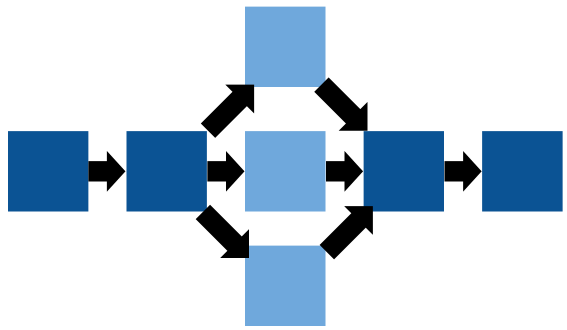
\includegraphics[width=\textwidth]{figures/3.png}
    \caption{A simple linear progression with a choice between three options halfway through.}
    \label{fig:simplegraph}
\end{figure}
%%%%%%%%%%%%%%%%%%%% Figure/Image 1 Ends here %%%%%%%%%%%%%%%%%%%%

If the experience is not designed to be replayed, we can consider each of the beats on a similar authoring level, effort-wise, because the player will encounter any of them a maximum of one time. However, if the work is designed to be heavily replayable, we want to prioritize the dynamism of the dark blue beats, as those are seen many times no matter what choice is picked in the middle. This plays into our next category: Reusability.

\subsubsection{Reusability}

When evaluating a potential experience's system design, we want to characterize how content can be reused, or how often content is common between playthroughs (if Replayability is a factor). As a general consideration, the more content is being reused, the heavier the lifting it's doing. This usually means the process intensity \cite{crawford1987process} will need to be higher, but that the quantity of required authoring (hopefully) is lower. However, the amount of different places content can be successfully reused depends on the work's Contextuality, which works in concert with this lens to either compound the Complexity requirement (as we'll see in Section \ref{sa-reusability} with \textit{Emma's Journey}) or facilitate Reusability if the amount of required Contextuality is relatively low.

\subsubsection{Contextuality}

One of the experience qualities that can impact authoring the most is its Contextuality. This category provides a useful lens for clarifying the relationship between the narrative and the state space of the game. For example, the authoring requirements for a narrative that contextually reacts to--and surfaces--a state-space of five boolean variables is very different from one that does so for fifty. Additionally, a narrative that reacts to game state that updates once a second is very different than one which only reacts once per player interaction, such as clicking a choice. High Contextuality experiences in this sense are more reactive and dynamic, though that dynamism of course comes with an authoring cost.

This lens is also useful for thinking about the dynamic juxtaposition of content for different intended narrative modes. We will explore this more thoroughly later in Section \ref{subsubsec:failbetter-and-qbn-systems} with Failbetter's concept of ``fires in the desert." For now it is enough to say that an experience in which an individual piece of content must make sense and support continuity from a previous one--such as narratives driven mostly by conversations between characters--poses a much higher Contextuality challenge than ones where each individual piece of content is a self-sufficient vignette. While the latter can rely on the player to fill in the context gaps and therefore has more leeway for Reusability, the former has a much higher standard for coherence (a dynamic we will elaborate upon in Section \ref{intro:controllability}) and as such can foreground a high amount of authorial burden.

\subsubsection{Summary}

These lenses help us evaluate a proposed narrative experience in terms of the player experience, with an eye towards clarifying issues that can impact the amount of authoring required to result in a completed media work. In general, the most challenging experiences will be ones in which the Explorability and Replayability of the play experience is high, the Reusability of authored content is low, and the Contextuality of content is high. However, even if the overall Traversability of a proposed experience is very high, it can still be tackled by relatively small teams of writers, given the proper tools and content design. This plays into the second component of the framework: Authorability.

\subsection{Authorability}

For Authorability, the overarching question is: how quickly / easily can content be created for the experience? For greater specificity, we break this down into the following four sub-questions:

\begin{itemize}
    \item \textbf{Proficiency}: what data format are authors required to work in? How technically demanding is that format?
    \item \textbf{Complexity}: how many different components does authoring a single piece of content entail?
    \item \textbf{Clarity}: how complex are the state/system dynamics that need to be kept in mind while authoring?
    \item \textbf{Controllability}: how difficult is it to create content which is reliably displayed in the intended manner when encountered by the player?
\end{itemize}

\subsubsection{Proficiency}

Proficiency is drawn primarily from Shneiderman's concept of ``direct manipulation'' \cite{shneiderman}, a useful lens for talking about authoring challenges for dynamic narrative systems. Essentially, direct manipulation is a goal for interfaces that can be used by novices easily, experts with fluency, and with a tight loop between an action taken in the tool, and its effect. 

Because dynamic narrative creation already requires authors to keep many things in mind (the characters, the story, the aesthetics, the ``possibility space'' of the narrative, all of which we will address shortly) we want to minimize the initial mental overhead for basic system-driven requirements as much as possible. Therefore, a system that has a low Proficiency requirement is desirable, within the restraints and requirements of other project variables. 

This is similar to the conclusion drawn by Spierling and Szilas in 2009, while assisting students authoring content for their dynamic narrative systems \cite{authoring_issues}. An additional note that plays into Proficiency as well, as they detailed, is that there is a ``vicious circle" in authoring for a system under active development. Authors may find they need new affordances in the course of content creation, which provoke changes to the underlying systems by engineers, which can then result in a higher Proficiency requirement, or a substantial change in content authoring that effectively erases any gained Proficiency due to new required syntax to support the added features.

Keeping Proficiency requirements low is particularly challenging with dynamic narrative experiences, because many times (as we'll see in the projects detailed in this dissertation) the surface text authoring needs to incorporate more advanced syntax, such as some sort of DSL (domain-specific language) to allow authors to specify different methods--state-driven or otherwise--the text may be reified and displayed. The design of these DSLs can potentially alleviate this if done with care, but ultimately depends wholly on the targeted Proficiency of the content authors. 

For example, imagine we need to write content for a character leaving a party. As authors, we know there are a couple different ways this can play out. Let's say they can leave amiably or angrily, depending on how well their conversations went. If we wanted to keep the required Proficiency low for authoring this content, we could have the systems person write a function that evaluates the conversations, and applies some formula resulting in ``positive" or ``negative." The author could then write something like \verb!_pn{That was nice.|That was terrible.}!. This sacrifices the author's ability to see or specify the conditions of what is a ``positive" or ``negative" state, for the ability to focus more on the text itself with a minimal amount of markup, and the capability to call that function despite a low Proficiency. If the author has higher Proficiency, we could risk exposing those conditions to them in a more complex DSL, which would give them higher individual authoring affordance, at the expense of requiring higher Proficiency (and higher Complexity, as we'll see in the following section).

\subsubsection{Complexity}

Hutchins et al. elaborated on Shneiderman's concept of direct manipulation as being the result of minimizing the \textit{Gulf of Execution} and the \textit{Gulf of Evaluation} \cite{Hutchins}, which have analogues with our notion of Complexity and Clarity. We use Complexity as a useful lens for characterizing the amount of effort necessary to take an action to achieve an authoring goal. The effort, as it applies to our targeted domain of content authoring, is characterized primarily through the complexity of data input required to create a singular piece of content. This problem is not new. Spierling and Szilas also encountered this with their authoring efforts, noting that ``even with graphical templates that help create the correct syntax, entering data takes time and prevents from quickly seeing the result of the created content" \cite{authoring_issues}.

While increases in Complexity are often unavoidable with increases in system expressiveness, it can be mitigated by proper tooling. Hutchins et al used a notion of \textit{semantic distance} to talk about how proper tools could close the Gulf of Execution: ``Semantic distance in the gulf of execution reflects how much of the required structure is provided by the system and how much by the user. The more that the user must provide, the greater the distance to be bridged" \cite{Hutchins}. 

Authoring tools which can aggregate disparate parts of the authoring process under one unified interface can decrease the semantic distance. For example, if a piece of content requires both surface text to be written, and semantic tagging to be applied to it to be understood by the game's process, one could lower the authoring Complexity by incorporating the authoring of both text and tags into one interface, as opposed to two disjoint ones. Another useful strategy is to incorporate the game's system dynamics such that invalid options cannot be authored, thus also reducing the semantic distance. For example, if a piece of content requires a reference to another piece of content, creating a field which automatically has valid options would decrease complexity, as opposed to requiring authors to look up reference IDs from another file. These HCI concerns can be generalized as a goal of ``making the commands and mechanisms of the system match the thoughts and goals of the user" \cite{Hutchins}. 

In general, we want Complexity to be as low as possible. This can be difficult with interactive narrative systems, because many times surface text authoring engages a different mindset than narrative design considerations of how / when / where said content is displayed. In practice, we can alleviate this by segmenting authoring tasks between the more system dynamics-focused narrative design tasks, and the aesthetic considerations of surface text authoring. However, care must be taken in the segmentation, as the separation of information and context can decrease Clarity for each component task, as we will detail in the following section.

\subsubsection{Clarity}

Paired with Hutchins et al's \textit{Gulf of Execution} is the \textit{Gulf of Evaluation}, which we partially incorporate as part of Clarity, and another part as Controllability (which we will detail in the next section). In general, we want the process-driven mechanics of content surfaced to the author as they're creating content, in as clear a manner as possible. We can do this by creating, as Hutchins et al say, an authoring interface that can ``present a good conceptual model of the system that is readily perceived, interpreted, and evaluated." For the three main projects detailed in this dissertation, this is mostly accomplished through data visualizations, which can place the content in context with playthroughs, or show the percentage of time particular content is displayed, and under what conditions. For works with a high amount of Contextuality, it is especially important that authors have Clarity in order to control how the content pieces are brought into juxtaposition with each other (as expanded in the next section on Controllability). 

For more lower-level concerns of surface text display, Clarity can be generally increased by providing ``live previews" of different ways the text may reify, and provide an easy way to see their expressive breadth. One tool particularly good at this is Compton's Tracery editor \cite{compton2015tracery}, which provides an easy way to specify the number of expansion iterations one wishes to see, and then expand out the authored context-free grammar to surface text. This leads to a tighter loop between evaluating the final text displayed, and the authoring of further dynamisms.

We want Clarity to be as high possible because without it, the link between the content and its dynamics is weakened. Especially for works which we want a high amount of Controllability (which is true of all the works detailed in this dissertation), low Clarity can mean either capitulating with simpler dynamics and conditions driving its display, or the risk of more surprising or uncontrolled juxtapositions, characterized as low Controllability.

\subsubsection{Controllability}
\label{intro:controllability}

Controllability describes how easy it is to create something with bad dynamics, or dynamics resulting in unexpected output. As a lens on Authorability, it's in dialogue with the type of generativity desired for the dynamic narrative. For example, works with higher Contextuality require higher Controllability for their authoring approaches, because the authors wish to achieve specific juxtapositions of content, though those juxapositions may be dynamically determined and generative.

To this end, as a general rule we always desire high Controllability for authoring, though the scale of what is ``high" or ``low" may differ work to work. Works which are more collage-like with lower Contextuality may have tooling support for ``high" levels of Controllability, which may prove inadequately low when applied to other works which demand much higher Contextuality, and thus Controllability.

The specific types of experiences we set out to create with the systems detailed in this dissertation were all ones in which we wanted a high amount of output control. Because of this, we chose symbolic AI approaches (known colloquially as ``good old-fashioned AI" \cite{haugeland1985artificial}). This is in contrast to a class of generative narrative and NLG (natural language generation) approaches which are connectionist, such as those driven by deep learning and machine learning methods \cite{gofai_vs_connectionist_1989}. While a great deal of research effort is rapidly advancing these methods, our emphasis on symbolic systems is motivated primarily by two preferences: syntactic guarantees, and output explainability.

Modern connectivist approaches are certainly generative and expressive, as demonstrated by GPT-2 \cite{radford2019language}, which some practioners have retrained to generate Borgesian wikis of fictional places \cite{book_of_endless_history} and retrained on even smaller corpuses to mimic specific styles, such as Branwen's work with poetry \cite{branwen_2019}. However, there is still a baseline of statistical invariance in the output that we wish to avoid. We want hard guarantees about the system output that is very difficult--if not currently impossible--for these models to provide, while still retaining their expressivity. Even models that ``bake in" control capabilities, such as Keskar et al's CTRL \cite{Keskar2019CTRLAC} (which parameterizes controls for style, content, and task-specific behavior) don't provide the type of fine-grained syntactic control we require for quality guarantees. On a more macro level, we're also focused on works which can maintain and control context over longer instances than a handful of paragraphs, an area that is being actively developed with approaches such as Sparse Transformers \cite{child2019sparsetransformer}, but is still nascent with such types of models.

Additionally, if we used these models and desired to change certain things to affect very specific qualities of specific output, we would run into issues trying to determine what to change in the model to accomplish our goals. While recent advances have been made to crack open the black box of machine learning models through XAI (explainable AI) approaches \cite{gunning2017explainable}, for the most part it is still very difficult to take generated output from these systems, and then come up with concrete steps that can be taken to change their output in highly defined ways.

Thus, while the approaches for the systems in this dissertation are driven by symbolic AI approaches for the abovementioned reasons, the overarching idea of Controllability can map to both symbolic and connectivist ones as well, as a lens to evaluate how rigorously authors must control the output of the system. This translates into higher authoring effort, through the increase in time spent evaluating the conditions that drive content display for the dynamic narrative system, whatever those may be.

\subsubsection{Summary}

The answers to these questions determine the difficulty of the task placed before content creators. If Authorability is low, even small-scale systems may suffer difficulties fielding playable experiences. However, maximizing Authorability by

\begin{itemize}
    \item lowering required Proficiency
    \item reducing authoring Complexity
    \item increasing authorial Clarity while writing for
    \item the level of Controllability appropriate to the experience
\end{itemize}

can help mitigate that. This typically is accomplished through the use of custom editors or other methodologies, and enables more content to be produced. Thus, experiences scoring high in overall Traversability with concomitant high authoring requirements can still be achievably created.

\section*{Related Frameworks}

This framework joins the ranks with other formalizations geared towards aligned but different purposes. Some of them apply to the general domain of game development, others more specifically to narrative games, and others still with content authoring for games.

\subsection{MDA Framework}

In thinking about the dichotomy of content (and its supporting systems) in dialogue with media experience requirements, the Authorial Leverage framework bears similarity to Hunicke and LeBlanc's MDA Framework \cite{hunicke2004mda}. Originally taught in workshops at the Game Developers Conference from 2001-2004 \cite{leblanc_2001}, the MDA Framework ``attempts to bridge the gap between game design and development, game criticism, and technical game research." It breaks down games into three categories: mechanics, dynamics, and aesthetics. Mechanics composes the procedures specifying the ``game-as-system", dynamics the run-time behavior of those procedures, and aesthetics the desired emotional responses evoked by those dynamics. These categories are intended as ``a lens or a view of the game -- separate, but causally linked" \cite{leblanc_2004}. These lenses are then used to inform the iterative design process--to help the game developer ``analyze the \textit{end result} to refine implementation, and analyze the \textit{implementation} to refine the result" \cite{hunicke2004mda}. The Authorial Leverage framework takes a similar tack, where the Traversability questions detailing the desired player experience frame the Authorability questions engaging with the implementation. However, compared to the more abstracted (and thus more generalizable) MDA Framework, the Authorial Leverage Framework is concerned solely with content authoring, and goes into more specific detail profiling how that is to be accomplished.

\subsection{System, Process, Product}

In 2010 Koenitz proposed a framework breaking down interactive dynamic narrative into three components: system, process, and product. Of these components, \textit{system} describes the ``digital artifact, as it exists on a digital storage medium combined with the hardware on which the artifact is executed", \textit{process} the ``actions of the user as interactor, and the opportunities provided by the system define and shape the process", and \textit{product} the completed playthrough produced by the user \cite{koenitz_framework}. This framework was created to find new ways to productively apply narrative theory to interactive digital narratives (abbreviated by Koenitz as IDN). This was motivated by Koenitz's feeling that IDNs are ``participatory transformational experiences", and that there is a key difference between ``the material artifact as a computer program and its output as a particular instantiation." As such, his framework is centered on the distinction between the system (both hardware and software) that enables the playthrough, and the playthrough itself. This is similiar to the Authorial Leverage framework's sub-categories of Explorability, Replayability, and Reusability, as those are similarly motivated to provide a lens to analyze content in terms of potential traversals, rather than a monolithic library.

\subsection{Axes of Analysis}

Three years later in 2013, Koentiz et al incorporated this with even more classification dichotomies, ranging from ``flexible / fixed" to ``script / procedural" and others. The goal of the different classification axes was to promote an analytical framework using ``processes based on small corpora and ad-hoc comparisons between select artifacts to visualize relevant characteristics" \cite{koenitz_idn}. This was in dialogue with previous categorization efforts such as Bevensee et al's PING (Passive-Interactive Narrative-Game) model \cite{aporia}. Bevensee et al created the PING model with its two axis--one for the dichotomy of game versus narrative, the other interactivity versus passivity--to position their work \textit{Aporia}, whose focus is communicating a narrative wholly through environmental storytelling. Koenitz et al's classifications also drew from Bura's proposed dichotomies of ``story versus system" and ``user control versus system control" \cite{koenitz_idn}.

While these types of analytical frameworks are admittedly more ad hoc, they are similarly motivated to the Authorial Leverage framework in that they're focused on providing flexible scaffolds that are based more on the utility they provide for thinking about particular aspects of given works, rather than claiming some sort of objective truth that applies to all dynamic narrative experiences. Additionally, as with PING, the Authorial Leverage framework arose from the abstracted insights derived from implementing specific works, and forming theories based on the experience of authoring with them, that can them be turned to other works to comparatively analyze them.

\subsection{PC3 Framework}

A year later in 2014, Magerko proposed the PC3 Framework, which was motivated by the desire to ``better understand how to dissect, compare, and contrast systems within similar as well as across different presentation media" \cite{magerko_PC3}. The range of ``different presentation media" is quite inclusive, spanning from complex computational narrative systems to simple story card games. The PC3 framework breaks down into the following components:

\begin{itemize}
    \item \textbf{P}: the computational \textit{processes} employed in the work
    \item \textbf{C}: the \textit{content} used in the system (as well as its narrative structure)
    \item \textbf{C}: the system of \textit{control} used to drive content display (centralized or de-centralized)
    \item \textbf{C}: the system's intended social \textit{context} or audience
\end{itemize}

Magerko's abstraction of process to encapsulate both computational and non-computational forms (such as the rules for tabletop games) allows it to juxtapose works that previously may have not been considered comparable. The content and control categories allow it to productively interrogate the surface-level content of works, the dynamics and design in how they are structured, as well as more top-level strategies, such as the use of planners (centralized control) or improv game rules (de-centralized). Lastly, the social context provides a way for the framework to account for the difference in audience for the completed experience. Magerko draws a distinction between the creation of works for training purposes, theatrical performances, or even between children and adults. This grounds the analysis in the pragmatics of its experience, much like the ``Product" in the System, Process, Product framework, or the Aesthetics of the MDA Framework.

PC3 and the Authorial Framework overlap in a few particular ways, although their ultimate aims are different. As with the System, Process, Product Framework, we find it useful to characterize the player's experience as a critical consideration in the system design. And certainly, both frameworks are concerned with dynamic content, and accounting for the dynamics their paired narrative structures entail. However, our Authorability Framework is geared more towards assisting the creators of said systems by providing a lens for strategic authoring decisions. In contrast, the PC3 Framework's focus is more for use by ``teachers, designers, and media theorists interested in the overlap between narrative systems (e.g. identifying the similarities and differences between the narrative systems behind Fiasco, Fa{\c c}ade and Dungeons \& Dragons)" \cite{magerko_PC3}.

\subsection{Progression Model}

New frameworks are continually being created, providing ever more tools for designers and theoriests to analyze interactive narrative works. In 2019, Carstensdottir et al proposed a ``descriptive framework developed to provide designers and practitioners with a common lexicon to describe and analyze their interactive narratives in terms of broad categories of elements that make up the interaction design" \cite{carstensdottir}. This model was derived from analysis of twenty-two games for their structure, progression mechanics, interaction modalities, and presentation. It is interesting to note that, with the exception of \textit{Prom Week} and \textit{Façade}, all were (to this author's knowledge) created by independent or AAA commercial game developers primarily with the singular goal of presenting a polished narrative experience, with no added research goals. Thus, Carstensdottir's model has its roots entirely in works motivated by a polished final experience. In the course of this analysis, Carstensdottir et al also formalized several authoring patterns in the work that they felt could be generalizable to other narrative forms.

Carstensdottir later developed this framework further into their Progression Model, which ``captures the narrative's structure from a users’ experience perspective", with a particular focus on capturing player progression in a graph-based representation called Progression Maps \cite{carstensdottir_diss}. In it, they identified five conceptual categories for interactive narrative design:

\begin{itemize}
    \item \textbf{Structure}: the typical graph-based representation of story progression
    \item \textbf{Progression Mechanics}: mechanics targeted towards player progression through the story
    \item \textbf{Interaction}: player affordance (such as input mapping and feedback)
    \item \textbf{Presentation}: narrative framing such that it impacts player interaction
    \item \textbf{Action Set}: the set of actions available to the player
\end{itemize}

This framework provides a valuable lens to analyze interactive narratives in terms of the user experience, which we are similarly interested in for determining a work's Traversability. However, our focus frames the player's affordance as the instigation point for authorial concerns, and our questions of Authorability, while informed by these questions of player affordance and game traversal, are meant more as a lens for practitioners to use in the course of creating new works.

\section{Contributions}

This dissertation contributes a new framework, the Authorial Leverage Framework, as an abstracted guide for analyzing dynamic narrative experiences (whether in progress or completed) and constructively talking about the authorial burden of their content creation. This framework also enables discussion about sustainably lowering the labor of such works while still preserving desired characteristics. This framework was abstracted from lessons learned in the implementation of three unique dynamic narrative systems, each of which tackles dynamic narrative in a categorically different way.

\begin{enumerate}
    \item \textbf{\textit{Ice-Bound}} creates dynamic narrative the player can sculpt until they arrive at a story of their choosing, through the unique affordances of a combinatorial narrative system.
    \item \textbf{StoryAssembler} marries a forward-search planner approach with a hierarchical task network (HTN) planner to afford greater flexibility in each individual unit of content, used to construct dynamic choice-based narratives.
    \item \textbf{\textit{Delve}} uses hierarchical ``story-sifting" to generate character narratives, and content-tagging coupled with an ontology to enable story manipulation through 3D objects in a first-person game.
\end{enumerate}

Each of these systems provides unique technical insights in their implementation. Furthermore, the process of authoring completed works with them (or in the case of \textit{Delve}, initial tool design to allow such authoring in the future) critically provided design insights that led to both authoring patterns which may be generalizable to other such dynamic systems, and methodologies for determining ``problem spots" in content dynamics, and how to avoid them. Critically, these insights could not have arisen from pure system implementation, only from the pragmatics of experience creation. Said insights are generalized into the Authorial Leverage Framework to facilitate content authoring, and will hopefully provide a useful lens to evaluate the development and design of future procedural narrative systems for others.

\section{Outline}
%%signposting%%
This dissertation explores three ``families" of dynamic narrative systems, through the implementation and content creation process for three separate projects: \textit{Ice-Bound}, \textit{Emma's Journey} (using the StoryAssembler system), and \textit{Delve}. For each, we first foreground the ``experience challenge" that we hoped to answer with said system. Prior works in a similar vein are then profiled, along with a targeted literature review for each system's area of research. For \textit{Ice-Bound}, this is combinatorial narrative. For StoryAssembler the focus is planner-driven systems and dynamic choice-based narrative systems. For \textit{Delve}, we turn to simulation narrativisation systems, computational metaphor systems, and ontology-driven systems. After laying this groundwork, we then dive into the technical details of each system's implementation, and content authoring procedures. 

Having established this, we then analyze each system and authoring approach in terms of the Authorial Leverage framework. We look at both content design decisions used to maximize each system's effectiveness, as well as authoring insights that may generalize to other systems in each family of experiences. Broadly speaking, \textit{Ice-Bound} shows how increasing Clarity is particularly useful for systems with high degrees of Explorability. For StoryAssembler, we focus on how works with high Contextuality require high Controllability, which can create authoring challenges, as seen in \textit{Emma's Journey}. 

Both \textit{Ice-Bound} and \textit{Emma's Journey} are completed experiences. For the last work, \textit{Delve}, we apply the framework to a work for which the systems are completed, but authoring has yet to begin in earnest. Through this, we show how a prospective application of the framework can provide useful guidance for maximizing authorial leverage while iterating on the system, and strategies to fall back on if it turns out the system requirements demand more authoring than we can feasibly provide. We then conclude with some overarching thoughts on the authoring experience across these three systems, and talk about future work in this area.
%%signposting%%